
\section{Modeling as Programming}
\label{sec:modeling-as-programming}

In this section we shall attempt to explore the argument that
modeling can be perceived as programming. We will do this through
a small collection of examples, illustrating how what is normally
considered as modeling can be perceived as programming. We start
with class diagrams, as found in UML and SysML, then move on to
a classical formal specification language such as VDM, and finally discuss the issues with domain-specific languages.

\subsection{Modeling of Class Diagrams}
\label{sec:complex-classes-in-scala}

A commonly used part of UML and SysML is the class diagram. The class diagram is a visualization of data structures as nodes and edges. Nodes represent data elements and edges represent the relationships between data elements. To take an
example, consider the class diagram in Figure \ref{fig:library}
(the example is adopted from \cite{?}). This diagram models libraries of books. In this diagram a box (node) denotes a type, a set of objects of that type. Hence for example \name{Library} denotes the type of libraries: a set
of library objects each denoting a library.
A library (top node) has a name, which is a string. Note that
such data of primitive types (strings, integers, reals, Booleans, ...) are represented as so-called {\em attributes} and are declared inside the boxes instead of as egdes, although in principle they are just edges to boxes representing primitive types. A library consists of (left arrow) 
a collection of books (zero or more represented by $0 .. *$),
reachable from the library via the field \name{books}. In the other direction: a book is related to zero or one ($0 .. 1$) libraries.
Similarly, a library (right arrow) has associated a collection of
members. Books and members have names. In addition each book has as
attribute the number of books on shelf. Finally, a loan is a connection between a book and a member. A library has associated
a collection of (current) loans.

\begin{figure}[ht]
\centering
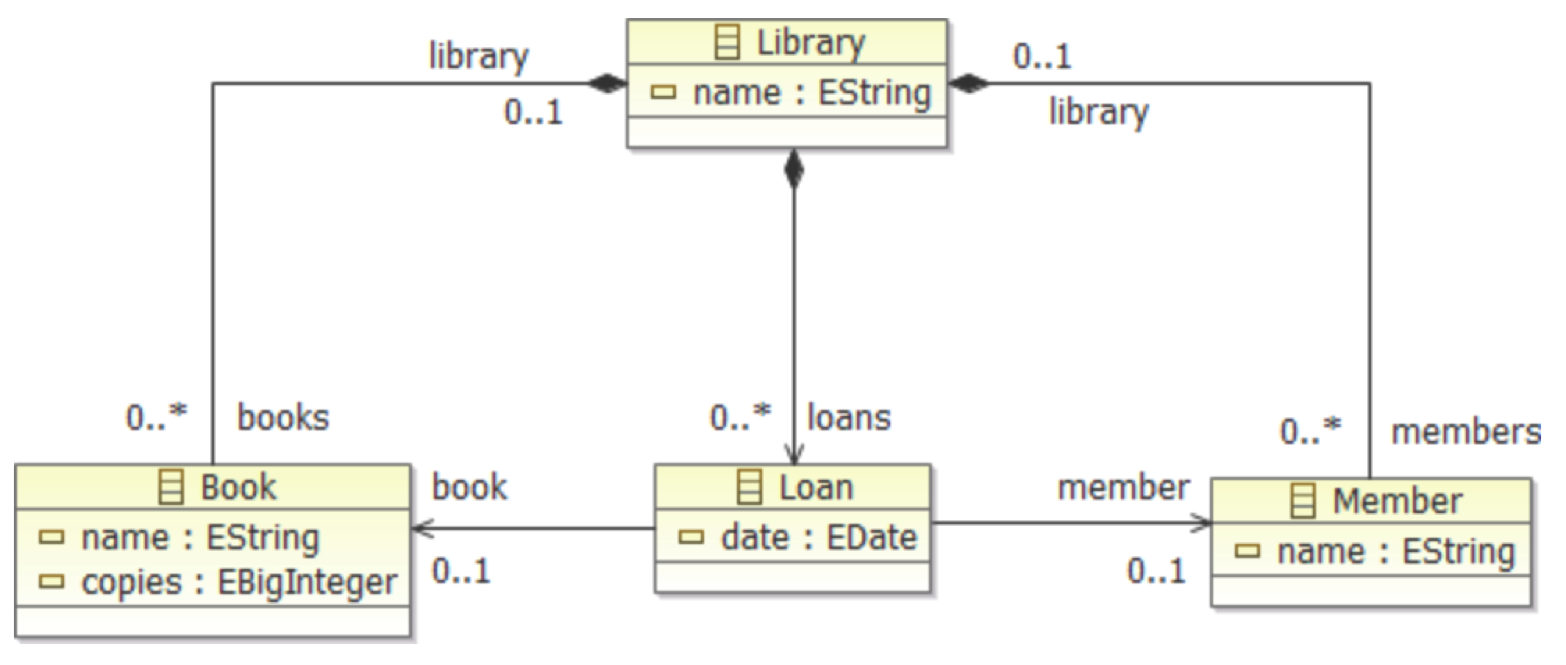
\includegraphics[width=0.9\textwidth]{images/library.png}
\caption{The book library}
\label{fig:library}
\end{figure}

In many modeling situations such diagrams form the core of the modeling effort. Constraints can be added to such diagrams.
For example one constraint could be that the number of copies of a book should be a number bigger than or equal to 1. Such a constraint can be added inside special constraint box on the diagram  in \ref{fig:library}, attached to the \name{Book} box
with a dotted line. It is interesting to note, that such a ``box''
with an associated constraint conceptually is very similar to the idea of a Z schema \cite{?}, as shown in Figure \ref{fig:book-z}\footnote{Note that the constraint can actually be avoided in Z by defining the type of \name{copies} to be $\mathbb{N}_1$, the natural numbers starting from 1.}.
This schema represents the fundamental concept of a model: a signature (the declaration of \name{name} and \name{copies} above the line with their types) and then zero or more axioms (below the line). 
%
Attempts have been made to provide textual versions of UML and SysML diagrams. An example is  the K specification language \cite{?}, that was developed at JPL. 
The expression language of K as well as Z 
(what is written in constraints) is predicate 
logic. Both languages support datatypes such as sets, including 
advanced set expressions such as set comprehension. K is object-oriented and is inspired by languages  such as Z, VDM \cite{?} and RAISE \cite{?}. 

Another alternative such textual notation is OCLInEcore \cite{?}, which is an attempt 
to define a textual language combining the Ecore model
of SysML with the OCL constraint language (Object Constraint Language) 
\cite{?}. OCL is a declarative expression language that is now part of the UML 
standard. OCL descended from Z, but is based on chained method calls read from left to right, starting from finite collections, in contrast to predicate logic. For example OCL does not have
general universal and existential quantification over infinite sets. In predicate 
logic we would write a universal quantification over a set/type 
$S$ as follows: $\forall x : S \bullet P(x)$. In OCL one would write this as:
\iocl{S->forAll(x | P(x))}. However, OCL requires $S$ to be finite,
in contrast to predicate logic, where $S$ can be infinite. This
is the major distinction between OCL and predicate logic, in addition to the alternative syntax. OCL is executable, given
a model instance.


%The \name{Book} class with the added constraint can be expressed in K as shown in Figure 
%\ref{fig:book-k}, very similar
%to the Z specification. 

\begin{figure}
\begin{schema}{Book}
	name: \seq CHAR \\
	copies: \num
\where
	copies > 0
\end{schema}
\caption{Z model of books in a library}
\label{fig:book-z}
\end{figure}

%\begin{figure}
%\begin{center}
%\begin{tabular}{c}
%\begin{lstlisting}[language=klang]
%class Book {
%  name : String
%  copies : Int
%   
%  req copies > 0
%}
%\end{lstlisting}
%\end{tabular}
%\end{center}
%\caption{K model of books in a library}
%\label{fig:book-k}
%\end{figure}

In order to illustrate OCLInEcore we expand our example by adding 
the requirement that ``{\em the number of loans that a book is part 
of should be less than or equal to the 
number of copies of the book}''. The following OCLInEcore model 
in Figure \ref{fig:book-oclinecore} formalizes this requirement.

\begin{figure}
\begin{center}
\begin{tabular}{c}
\begin{lstlisting}[language=oclinecore]
class Book {
  attribute name : String;
  attribute copies : Integer;

  property library#books : Library[?];
     
  property loans : Loan[*] { derived }
  {
    derivation: library.loans->select(book=self);
  }

  operation isAvailable() : Boolean[?]
  {
    body: loans->size() < copies;
  }
     
  invariant CopiesPositive:
    copies > 0;
     
  invariant SufficientCopies:
    library.loans->select(book=self)->size() <= copies;     
}
\end{lstlisting}
\end{tabular}
\end{center}
\caption{OCLInEcore model of books in a library}
\label{fig:book-oclinecore}
\end{figure}

In addition to the two attributes \name{name} and \name{copies},
two properties and an operation is defined, all of which are used 
to express the new invariant. In contrast to an {\em attribute}, 
which has a primitive type, a {\em property} is linked to one or 
more objects of another user-defined 
type (those drawn as boxes in class diagrams).
The property \name{library} links a book to the library it is part 
of, and is the ``{\em opposite property}'' of the \name{books} 
property of the \name{Library} (expressed using the \iocl{#}-
notation), meaning that of a book is in the \name{books} set (a bag 
in fact) of a library, then the library is also in the 
\name{library} of the book. The `\iocl{?}' represents 0 or 1.

The property \name{loans} denotes a collection of \name{Loan} 
objects and is 
derived (meaning its value depends on other values), with the 
formula defining 
its value provided as an OCL expression.
The expression reads as follows: from this book (referred to as 
\iocl{self} later in the expression), retrieve the library it is 
part of, retrieve the 
loans of this library, and select those for which the book is equal 
to \iocl{self}. For a given collection \iocl{S}, the notation 
\iocl{S->M(...)} 
means calling the method \iocl{M} on the set \iocl{S}. Hence in 
this case the
\iocl{select(predicate)} method is defined on sets and returns the 
subset of 
elements of the set satisfying the predicate.
The operation \name{isAvailable} returns a Boolean, and is defined 
by retrieving the loans as a collection, evaluate its size, and 
compare to the 
number of copies available. Finally, the two invariants can be 
formulated, and their explanation should at this point be straight 
forward.

The main point we are trying to make here is that the OCLInEcore model, which in reality is very similar to a Z specification (signature + axioms), can (for the most part) be elegantly expressed in the Scala programming language. This is shown in Figure \ref{fig:book-scala}. The class \iscala{Book} extends the
class \iscala{Block}, which offers various methods for writing models, including the \iscala{invariant} method uses to define invariants. What in the OCLInEcore model was the property \iscala{loans} and the operations \iscala{isAvailable}, are here modeled as methods (using the \iscala{def} keyword). Multiplicities such as \iocl{Loan[*]} are modeled using Scala's collection libraries, in this case \iscala{Set[Loan]}. The Scala definitions should be somewhat obvious. It is clear that Scala in this case
can model this problem as well as OCLInEcore. In addition, Scala offers so much more than OCLInEcore, such as an actual programming language.

\begin{figure}
\begin{center}
\begin{tabular}{c}
\begin{lstlisting}[language=scala]
class Book extends Model {
  var name: String
  var copies: Integer
  var library: Library

  def loans: Set[Loan] =
    library.loans.filter(_.book eq this)

  def isAvailable(): Boolean =
    loans.size < copies
      
  invariant("CopiesPositive") {
    copies > 0
  } 
       
  invariant ("SufficientCopies") {
    library.loans.filter(_.book eq this).size <= copies
  }       
}
\end{lstlisting}
\end{tabular}
\end{center}
\caption{Scala program modeling books in a library}
\label{fig:book-scala}
\end{figure}

\begin{figure}[htb]
\begin{center}
\begin{tabular}{c}
\begin{lstlisting}[language=scala]
   class Model {
     type Constraint = Unit => Boolean

     var constraints: List[(String, Constraint)] = Nil

     def invariant(c: => Boolean) {
       constraints ::= ("", (Unit => c))
     }

     def invariant(name: String)(c: => Boolean) {
       constraints ::= (name, (Unit => c))
     }

     def evaluate() {
       for ((n, c) <- constraints) assert(c(), n)
     }
   }
\end{lstlisting}
\end{tabular}
\end{center}
\label{fig:invariant-scala}
\caption{Support for defining invariants in Scala}
\end{figure}

The only code that has to be written to provide support for writing
class invariants is the definition of the class \iscala{Block}, which is shown in Figure \ref{fig:invariant-scala}. Without going into details, the class defines a method \iscala{invariant},
which as argument takes a Boolean call-by-name argument 
The argument is not evaluated before the method is called, 
rather, it is only evaluated whenever referred to. In this case
it is stored, still unevaluated, in a list of invariants, all
of which can then be evaluated with a call of \iscala{evaluate}.


\subsection{VDM Specifications}
\label{sec:vdm-in-scala}

As another example, we shall consider a a chemical plant alarm management system, first modeled in \vdmpp{} in \cite{vdmplusplus05} and also modeled in Scala in 
\cite{?}. We show here a slight modification of 
the \vdmpp{} specification as well as the 
corresponding Scala program. In \cite{vdmplusplus05}
the example specification was associated with 
a corresponding UML class diagram to illustrate how the two
techniques can co-exist. Here we shall put emphasis on
\vdmpp{} and its relationship to Scala.

The system shall manage the calling out of experts to deal with 
operational faults discovered in a 
chemical plant. 
Two operations must be provided.
\name{ExpertToPage}: Upon detection of a faulty condition, an alarm is raised, and an expert on duty is assigned to
handle the alarm. Each alarm is associated with a specific 
qualification required to fix the causing
problem, and each expert is associated with a set of 
qualifications. Upon an alarm, an expert must be found, and paged, 
that is on duty during the corresponding period and with the right qualification.    
\name{ExpertIsOnDuty}: return the periods on which an expert is on duty.      
In addition, the state of the system must satisfy the following
{\em invariant}:
(i) There must be experts on duty during all periods 
allocated in the system. 
(ii) For any alarm and for any period, there should exist an expert assigned to that period that has the qualification required
to fix the source problem of the alarm.

The \vdmpp{} class \name{Plant} in Figure \ref{fig:plant-vdm} 
is part of the model of this system (other classes/types shown in
\cite{vdmplusplus05} have been left out here: 
\name{Alarm}, \name{Period}, and \name{Expert}).
The body of this class is divided into three sections: {\em instance variables} (mutable variables), {\em functions} (with no side-effects) and {\em operations} (with side-effects). An invariant defined by the function \name{PlantInv} is imposed on the instance variables. We shall not go into the further details
but just refer to the corresponding Scala program modeling the plant in Figure \ref{fig:plant-scala}.

\begin{figure}
\begin{center}
\begin{tabular}{c}
\begin{lstlisting}[language=vdm]
class Plant
  instance variables
    alarms : set of Alarm;
    schedule : map Period to set of Expert;
    
    inv PlantInv(alarms,schedule);

 functions
    PlantInv: set of Alarm * map Period to set of Expert -> bool
    PlantInv(as,sch) ==
      (forall p in set dom sch & sch(p) <> {}) and
      (forall a in set as &
         forall p in set dom sch & 
           exists expert in set sch(p) &
             a.GetReqQuali() in set expert.GetQuali());

  operations
    public ExpertToPage: Alarm * Period ==> Expert
    ExpertToPage(a, p) ==
      let expert in set schedule(p) be st
        a.GetReqQuali() in set expert.GetQuali()
      in
        return expert
    pre a in set alarms and p in set dom schedule
    post let expert = RESULT in
      expert in set schedule(p) and
      a.GetReqQuali() in set expert.GetQuali();
		
		 
    public ExpertIsOnDuty: Expert ==> set of Period
    ExpertIsOnDuty(ex) ==
      return {p | p in set dom schedule & ex in set schedule(p)};
end Plant
\end{lstlisting}
\end{tabular}
\end{center}
\caption{VDM++ model of plant}
\label{fig:plant-vdm}
\end{figure}

\begin{figure}
\begin{center}
\begin{tabular}{c}
\begin{lstlisting}[language=scala]
trait Plant extends Model {
  var alarms: Set[Alarm]
  var schedule: Map[Period, Set[Expert]]

  invariant{PlantInv(alarms, schedule)}

  def PlantInv(alarms: Set[Alarm], schedule: Map[Period, Set[Expert]]): Boolean =
    (schedule.keySet forall {p =>  schedule(p) != Set() }) &&
      (alarms forall { a =>
        schedule.keySet forall { p =>
          schedule(p) exists { expert =>
            a.reqQuali in expert.quali
          }
        }
      })


  def ExpertToPage(a: Alarm, p: Period): Expert = {
    require((a in alarms) && (p in schedule.keySet))
    schedule(p) suchthat { expert =>
      a.reqQuali in expert.quali
    }
  } ensuring { expert =>
    (a.reqQuali in expert.quali) &&
      (expert in schedule(p))
  }

  def ExpertIsOnDuty(ex: Expert): Set[Period] =
    schedule.keySet filter { p => ex in schedule(p) }
}
\end{lstlisting}
\end{tabular}
\end{center}
\caption{Scala program modeling plant}
\label{fig:plant-scala}
\end{figure}

\subsection{Domain Specific Languages}
\label{sec:dsl-in-scala}


